\vfill
\clearpage
\appendix

\stepcounter{section}
\hfill ПРИЛОЖЕНИЕ А
\begin{center}
  \textbf{Пример проверки сводимости}
\end{center}
\markboth{\MakeUppercase{}}{}
\addcontentsline{toc}{section}{Приложение А. Пример проверки сводимости}

\begin{figure}[h!]
  \centering
  \begin{subfigure}{\linewidth}
    \centering
    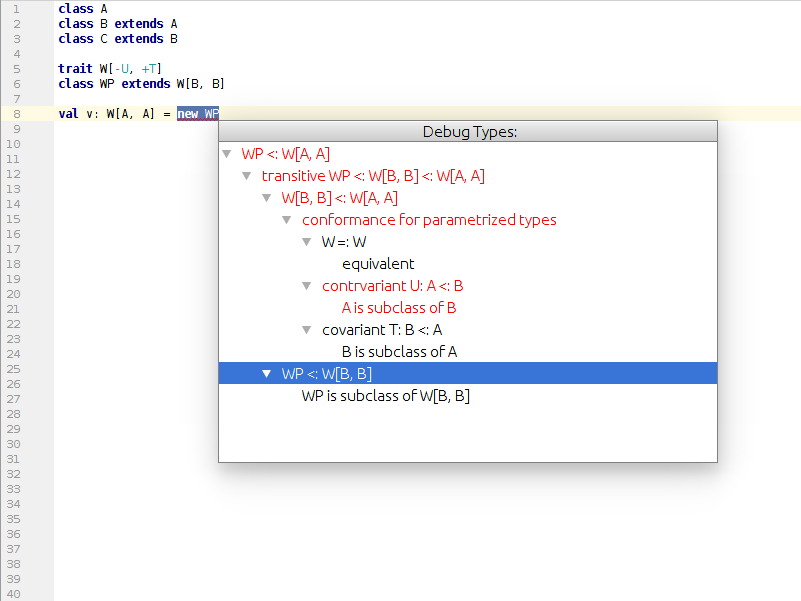
\includegraphics[width=.8\linewidth]{img/conformance1}
    \caption{Неправильное сведение}
  \end{subfigure}

  \begin{subfigure}{\linewidth}
    \centering
    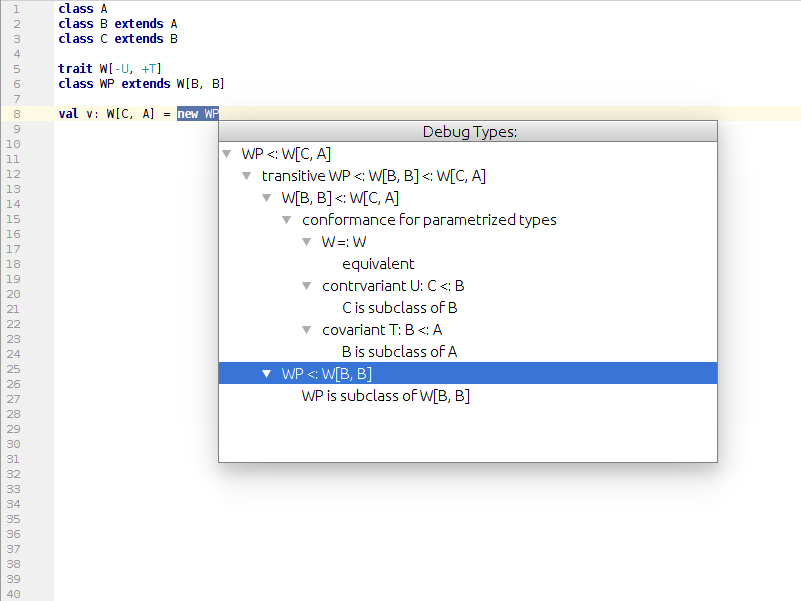
\includegraphics[width=.8\linewidth]{img/conformance2}
    \caption{Правильное сведение}
  \end{subfigure}
  \caption{Проверка сводимости}
  \label{fig:conformance}
\end{figure}


\vfill
\clearpage
\newpage


\vfill
\clearpage
\appendix

\stepcounter{section}
\hfill ПРИЛОЖЕНИЕ Б
\begin{center}
  \textbf{Пример вывода типов}
\end{center}
\markboth{\MakeUppercase{}}{}
\addcontentsline{toc}{section}{Приложение Б. Пример вывода типов}

\begin{figure}[h!]
  \centering
  \begin{subfigure}{\linewidth}
    \centering
    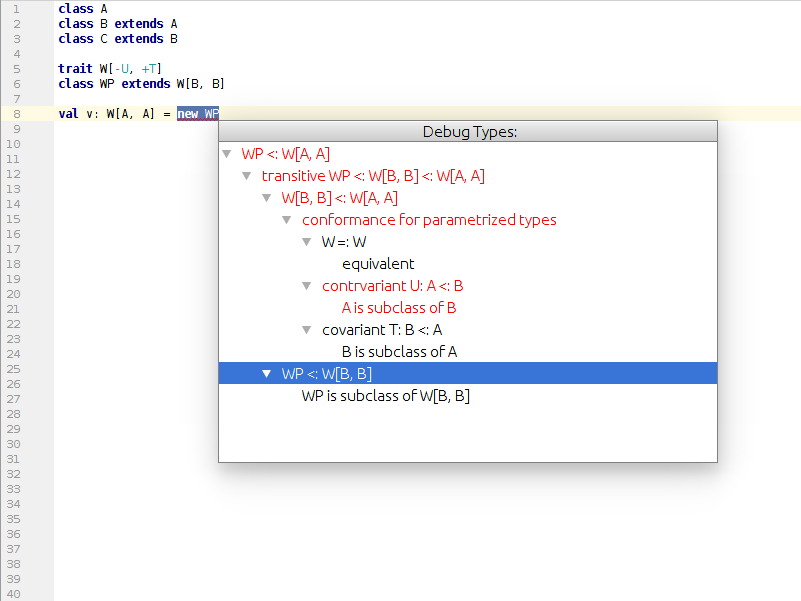
\includegraphics[width=.8\linewidth]{img/conformance1}
    \caption{Неправильное сведение}
  \end{subfigure}

  \begin{subfigure}{\linewidth}
    \centering
    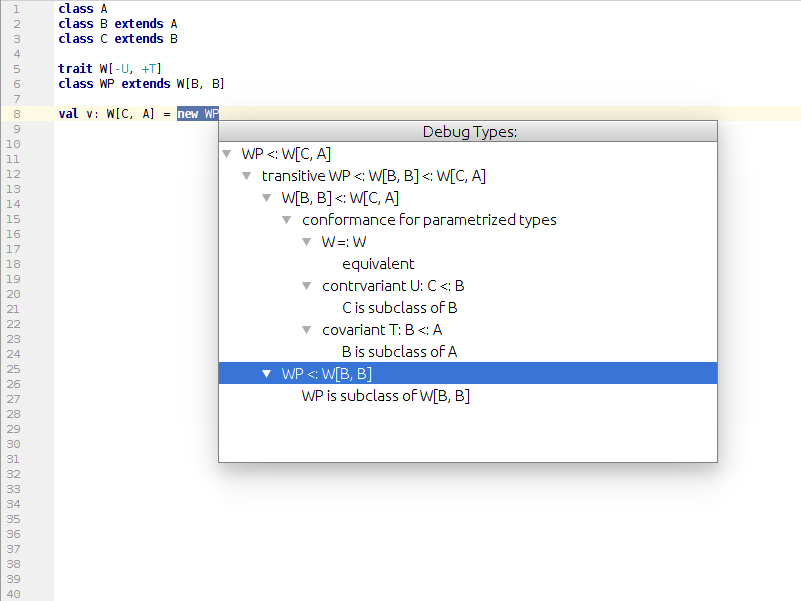
\includegraphics[width=.8\linewidth]{img/conformance2}
    \caption{Правильное сведение}
  \end{subfigure}
  \caption{Проверка сводимости}
  \label{fig:infer}
\end{figure}


\vfill
\clearpage
\newpage


\vfill
\clearpage
\appendix

\stepcounter{section}
\hfill ПРИЛОЖЕНИЕ В
\begin{center}
  \textbf{Пример выбора перегрузки функции}
\end{center}
\markboth{\MakeUppercase{}}{}
\addcontentsline{toc}{section}{Приложение В. Пример выбора перегрузки функции}

\begin{figure}[h!]
  \centering
  \begin{subfigure}{\linewidth}
    \centering
    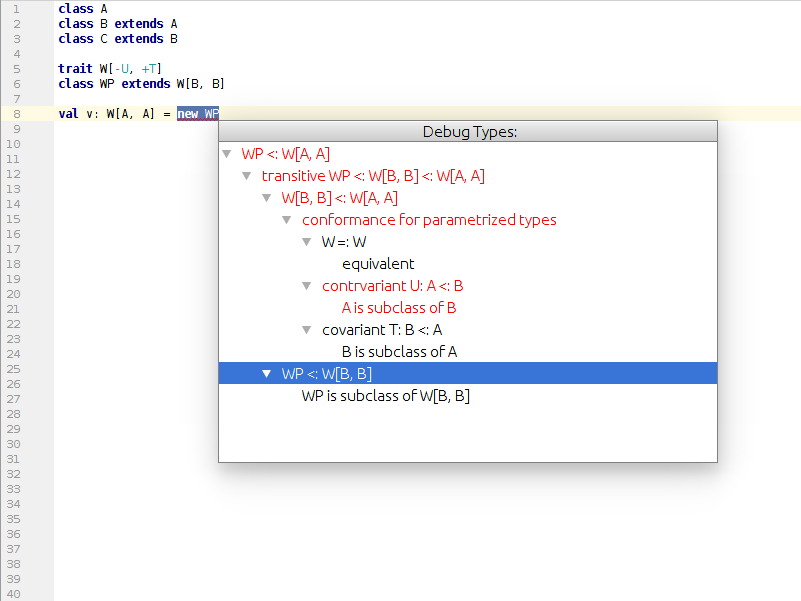
\includegraphics[width=.8\linewidth]{img/conformance1}
    \caption{Неправильное сведение}
  \end{subfigure}

  \begin{subfigure}{\linewidth}
    \centering
    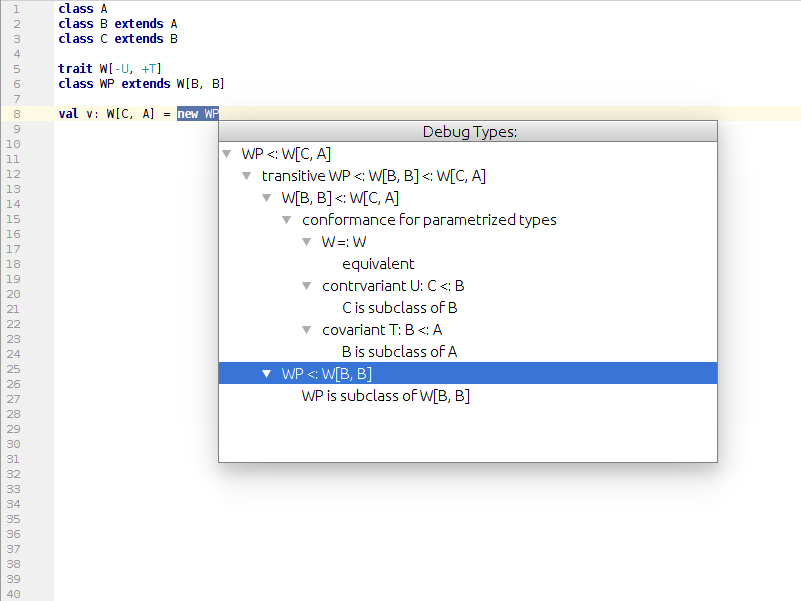
\includegraphics[width=.8\linewidth]{img/conformance2}
    \caption{Правильное сведение}
  \end{subfigure}
  \caption{Проверка сводимости}
  \label{fig:overloading}
\end{figure}
